\subsection{Mirror re-coating}

As seen in \F{optics}, each LTCC segment is composed of four optical surfaces: one elliptical mirror,
one hyperbolic mirror, one cylindrical mirror, and the Winston cone.
The reflectivity of a random selection of 30 elliptical, cylindrical and hyperbolic mirrors from two sectors was measured.
All the mirrors analyzed showed significant degradation from the original desired reflectivity of 90$\%$ in the visible spectrum,
see for example \F{reflectivityBefore}.
A refurbishment of the mirrors was crucial to enhance the detector response to the pion emitted Cherenkov light.
Due to the material, assembly, and dimensions of the different types of mirrors, two different techniques were applied to refurbish the
reflective surfaces.

\begin{figure}
\centering
	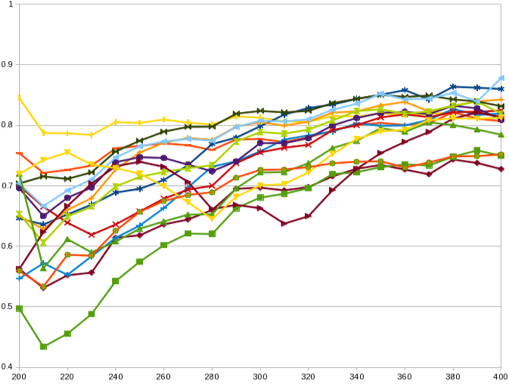
\includegraphics[width=1.0\columnwidth,keepaspectratio]{img/mirrorsReflectivityBefore.png}
	\caption{Reflectivity measurement as a a function of wavelength of a sample of 8 mirrors before re-coating, each sampled at two different places (front and back). The reflectivity
				was measured using a monochromator (Newport model CS260-USB-1-FH-A) with a deuterium light source with a reach
            between 200 nm and 400 nm. The reflectivity showed a degraded quality of about 65$\%$ instead of an optimal 90$\%$.}
	\label{fig:reflectivityBefore}
\end{figure}


\subsubsection{Re-coating of cylindrical mirrors}

The cylindrical mirrors range from 6 to 12 inches in length. Each mirror is made from a single piece of aluminum or plastic.
Due to the small size, they fit in most vacuum chambers used to coat mirrors by evaporation of aluminum with magnesium fluoride
(AlMgF$_2$). After successful testing of re-coating of AlMgF$_2$ onto the existing substrate, the work of re-coating 216 cylindrical mirrors
was awarded to ECI~\cite{ECI}. See \F{reflectivityAfter} for typical reflectivity values after re-coating.

\begin{figure}[h]
	\centering
	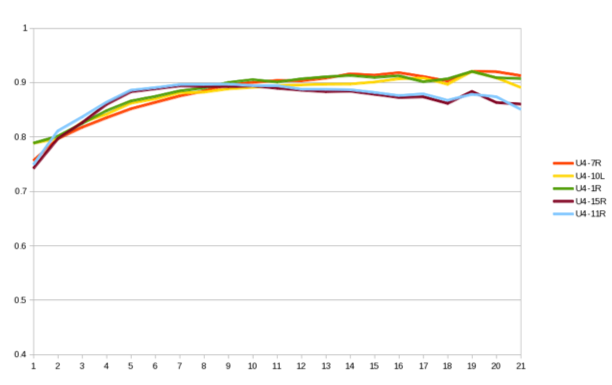
\includegraphics[width=0.95\columnwidth,keepaspectratio]{img/mirrorsReflectivityAfter.png}
	\caption{Reflectivity measurement as a function of wavelength of a sample of 5 mirrors measured after gluing the Lexan strips (see text for detail).
            Note the very high value of reflectivity in the UV region, where most of the Cherenkov light is produced. In the visible spectrum,
            the reflectivity is about 90$\%$.}
	\label{fig:reflectivityAfter}
\end{figure}

\subsubsection{Re-coating of elliptical and hyperbolic mirrors}

The elliptical and hyperbolic mirrors are composed by a Kevlar support structure with a Lexan substrate. The mounting hardware
material, which allowed for pitch, roll, and yaw alignment of the mirrors, included wood and aluminum that was glued to the support structure.

Several companies attempted to re-coat these mirrors but failed due to the outgassing of the various materials. Furthermore, many of the mirrors
are $>$1 m in length, longer than most vacuum chambers. Therefore the AlMgF$_2$ could not be re-deposited directly on the mirrors.

A different approach consisted of coating thin (25 $\mu m$) Lexan strips and gluing the strips onto the mirror substrate. While promising, this
presented the challenge of protecting the coated Lexan strip from shipping and handling and from the gluing procedure to the mirrors.

A working chain was setup to:

\begin{enumerate}
	\item coat the Lexan strip
	\item protect with a temporary film for shipping and handling
	\item ship to Jefferson Lab
	\item glu to mirror substrates
	\item remove the protective film
	\item test reflectivity
\end{enumerate}

An example of unwrapping the film off the Lexan strip is shown in \F{filmOnStrip} (top). Several companies produced various test samples with
various protective material films. The job was eventually awarded to ECI \cite{ECI}.
%The setup to glue the coated Lexan strip onto the existing mirrors is shown in \F{filmOnStrip} (bottom).
After 24 hours of curing time the film was removed.
The typical reflectivity of the refurbished mirrors is shown in \F{reflectivityAfter}.


\begin{figure}[ht]
\centering
	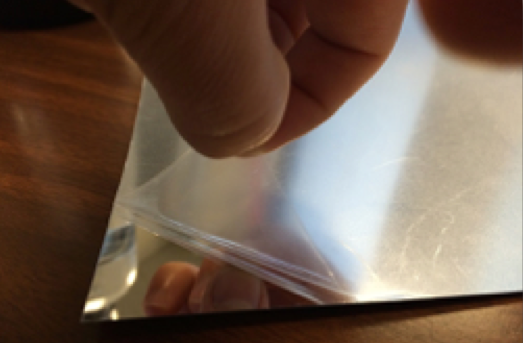
\includegraphics[width=0.98\columnwidth,keepaspectratio]{img/filmOnStrip.png}
	\caption{The protective film. For the elliptical and hyperbolic mirrors the Lexan strips were coated with AlMgF$_2$
				and covered with films to protect the handling and the
				gluing on top of the mirrors. The photo shows the process of removing the
            protecting film from one such strip. The surface reflectivity was tested immediately after the installation on the substrate and again
            48 hours after that. Only the samples from ECI \cite{ECI} resulted in a consistent high reflectivity. }
	\label{fig:filmOnStrip}
\end{figure}


\subsubsection{Elliptical mirrors gaps}

The segment with long elliptical mirrors presented several gaps between them, some a few cm long. To make sure that no light is lost in these gaps,
additional 120 $\mu$ m thick Lexan extensions coated with AlMgF$_2$ were glued to cover the gaps. The strips were manufactured by ECI~\cite{ECI}.


\subsubsection{Mirror re-coating summary and results}

All 216 cylindrical mirrors were re-coated on the existing surface. All 216 elliptical and 216 hyperbolic mirrors were refurbished using Lexan strips
coated with AlMgF$_2$ glued onto the substrate. The different sizes of the mirrors were accounted for using different widths for the Lexan strips, see
summary Table~\ref{tab:strips}.


\begin{table}[h]
	\begin{center}
		\begin{tabular}{| l | c |}
			\hline \hline
			Quantity  & Description \\
			\hline
			190       & 9" x 36" x 0.010” coated sheet    \\
			150       & 10" x 36" x 0.010” coated sheet   \\
			6         & 10" x 36" x 0.010” coated sheet   \\
			\hline \hline
		\end{tabular}
	\end{center}
	\caption{Summary of material used for the elliptical and hyperbolic mirrors. The total length of the Lexan strip necessary to re-coat the 216 elliptical
            and 216 hyperbolic mirror was 310 meters.}\label{tab:strips}
\end{table}


In \F{reflectivityAfter} a typical spectrum of reflectivity that applies to all cylindrical, elliptical and hyperbolic mirrors is shown.
The re-coated mirrors shows a $\sim 90\%$ reflectivity in the visible spectrum and an exceptional $\sim 80\%$
reflectivity in the UV spectrum.



\subsection{Mirrors alignment}

A new procedure was developed to align the mirrors with the LTCC boxes that takes advantage of their focusing capabilities.
The elliptical mirror focal points (see \F{alignmentSimulation}) are 1. the target (origin of the lab coordinate system)
and 2. a point behind the hyperbolic mirror. The focal points if the hyperbolic mirrors are 1. a point near the focal point of the elliptical mirrors and
2. above the face of the PMTs.

The geometrical shape of the mirrors has been built into the Geant4 simulation. When a laser line coming from the target is directed at the mirror,
it is focused on the hyperbolic focal point, then directed at the PMT, see \F{alignmentSimulation}.
This geometrical focusing was used during the mirror alignment: a 3 mW, 635 nm laser was placed, relative to the detector,
in center of the CLAS coordinate system, the location of the liquid hydrogen target and first ellipse focal point.
The laser was mounted on a structure that allowed the beam direction and line angle to move with respect to the floor, while keeping
the origin of the laser at the coordinate system origin.
This position was accurate at the 0.5 mm level. The laser was spread through two cylindrical lenses onto a laser line and shone
longitudinally along the center line of each elliptical mirror. Both the elliptical and hyperbolic mirrors were then adjusted in pitch, roll, and yaw to minimize the light spot
dimensions and to center it in the middle of the face of the PMT.


\begin{figure}[ht]
\centering
	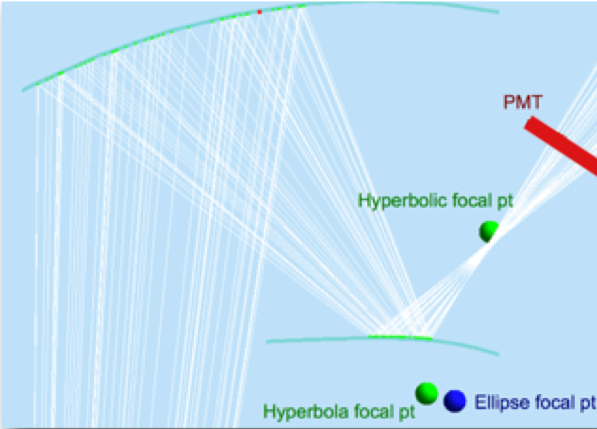
\includegraphics[width=0.95\columnwidth, keepaspectratio]{img/mirrorAlignmentSimulationZoomed.png}
	\caption{The simulation of a laser line (white tracks are photons) originating from the target (first ellipse focal point) and directed at the elliptical mirrors. The photons are reflected
		      to the second ellipse focal point. The hyperbole first focal point is near the ellipse focal point so the hyperbolic mirror
			   reflects the incoming photons to the hyperbole second focal point, located above the face of the PMTs.
			   This picture illustrate the procedure used for the alignment: the mirrors positions are adjusted until the laser line originating from the target is focused on the face of the PMT.}
	\label{fig:alignmentSimulation}
\end{figure}


%\begin{figure}
%\centering
%	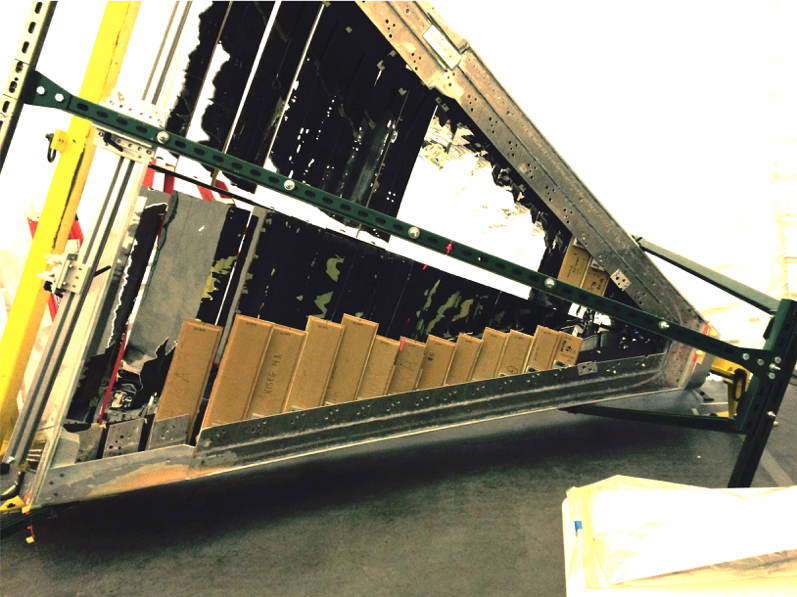
\includegraphics[width=0.95\columnwidth, keepaspectratio]{img/laserAlignment1.png}
%	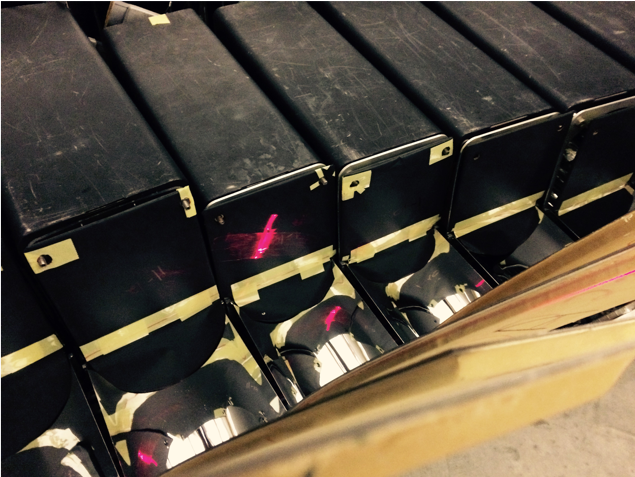
\includegraphics[width=0.95\columnwidth, keepaspectratio]{img/laserAlignment2.png}
%	\caption{The laser alignment setup. Top: the laser was placed, relative to the detector, in the lab coordinate system. The laser line was shined on each elliptical mirror.
%         Bottom: zoomed in view of the laser line focused on the center of the PMT after the mirrors were aligned.}
%	\label{fig:laserAlignment}
%\end{figure}

